\section{Power-train modeling}
This section covers the specific modeling approaches used for each powertrain component. Figure \ref{fig:Tractor_Powertrain} shows an overview of the major powertrain components denoted as squares. Inputs to the engine and powertrain are shown as circles.  
\begin{figure}[h]
    \centering
    \includegraphics[width=4in]{Tractor_Powertrain}
    \caption{Diagram of major MT865 tractor powertrain components \cite{Caterpillar2002,alexander1987caterpillar}. Inputs are denoted in red circles as the throttle $\Pi$, gear selection $g_{GR}$ and the hydraulic pump command $D_P$ which linearly maps to the driver's steering angle $\alpha$ in eq. \ref{eq:steerr2pump}.}
    \label{fig:Tractor_Powertrain}
\end{figure}
\subsubsection{Engine Model}
The engine model is created by fitting a 3rd order polynomial to torque-speed engine data, which is provided in \cite{Caterpillar2002}. Figure \ref{fig:Engine_Curve} shows the resulting model for an MT865 Challenger Model Tractor. The engine model is valid for the allowable operating engine speed range, i.e., engine speed $\Omega \in [1300, 2300]$ RPM. The polynomial curve fit is referred to as an engine torque or engine power demand function $g(\Omega)$ and provides the maximum amount of power available at a given engine speed whose form is given by
\begin{linenomath*}
    \begin{equation}\label{eq:power_demand_function}
        g(\Omega) = P_{max}(a\Omega_N + b\Omega_N^2 - c\Omega_N^3)
    \end{equation}
\end{linenomath*}
\begin{linenomath*}
    \begin{equation}\label{eq:n_define}
        \Omega_N \equiv \frac{\Omega}{\Omega_0}
    \end{equation}
\end{linenomath*}
where $a$, $b$, and $c$ are fitted polynomial coefficients, $P_{max}$ is the point of maximum power on the engine torque-speed curve and $\Omega_0$ is the engine speed at which it occurs \cite{MathWorks2015GenericEngine}. The total output power from the engine is $P(\Omega,\Pi) = \Pi g(\Omega)$ where $\Pi \in [0,1]$ is the normalized throttle command. The torque demand function is then given by
\begin{linenomath*}
    \begin{equation}\label{eq:engine_torque}
        \tau_e = \Pi\frac{P_{max}}{\Omega_0}\frac{a\Omega_N + b\Omega_N^2 - c\Omega_N^3}{\Omega_N}
    \end{equation}
\end{linenomath*}
The governor is modeled as supplying zero engine torque if the engine is operating above its maximum allowable speed. It should be noted, however, that if the engine operates in this region, it can be costly with regard to simulation times. Therefore, a hyperbolic tangent function is used to taper down the throttle at higher engine speeds providing an equation for the throttle signal delivered to the engine
\begin{figure}[tb]
    \centering
    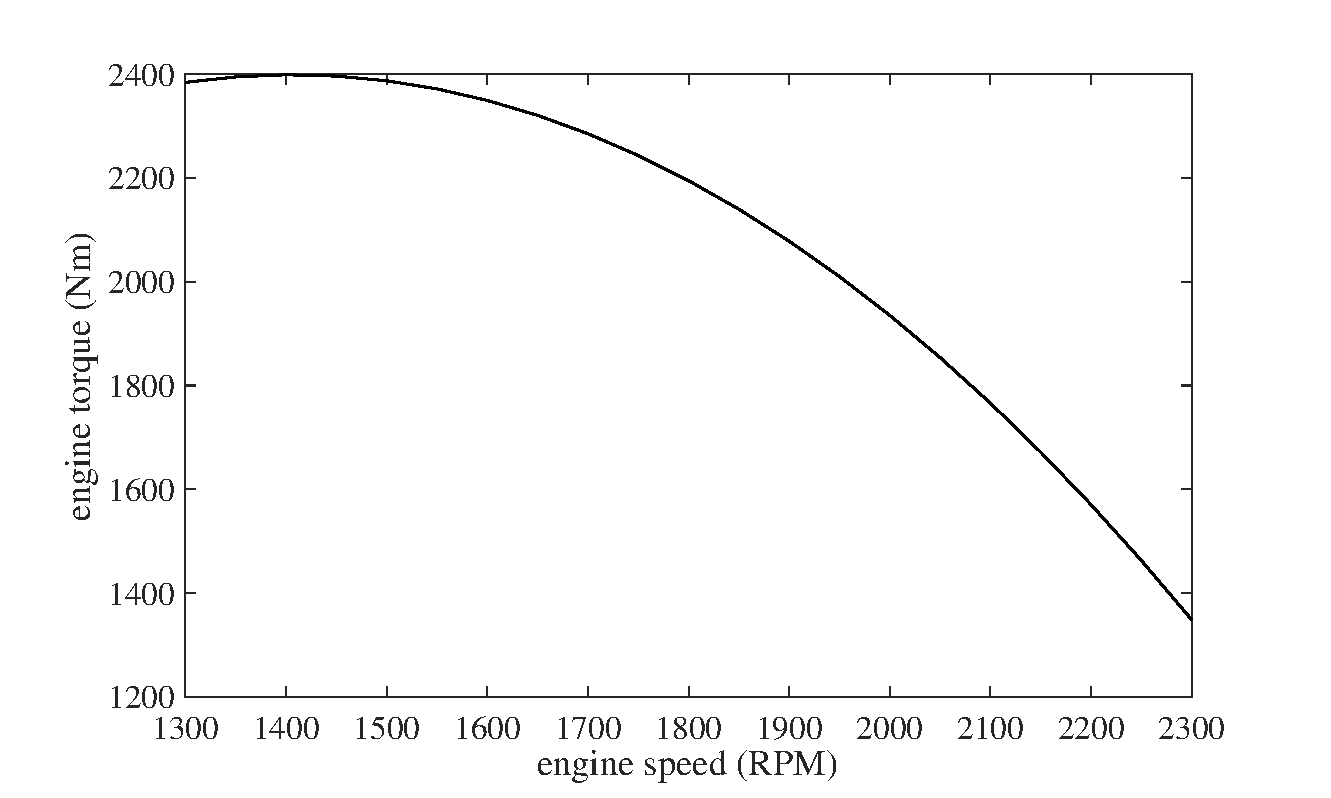
\includegraphics[width=3.5in]{Engine_Curve}
    \vspace{-5pt}
    \caption{Plot of the torque demand function in eq. \ref{eq:engine_torque} for the engine model of an MT865 tractor. During operation, this function determines the maximum amount of torque $\tau_{E,Max}$ that can be commanded. To command $\tau_{E,Max}$, a throttle $\Pi = 1$ is required.}
    \label{fig:Engine_Curve}
\end{figure}
\begin{linenomath*}
    \begin{equation}\label{eq:throttle_taper}
        \Pi := \Pi\tanh\Bigg(\frac{|2300-\Omega|(2\pi/60)}{\chi}\Bigg)
    \end{equation}
\end{linenomath*}
The parameter $\chi$ allows for the function to be dilated and controls how close to the maximum engine speed the engine will operate.

\subsubsection{Direct Drive System}
In order to simulate start-up, it is necessary to include a torque converter or direct drive mechanism in simulations since engine speeds do not match transmission shaft speeds in this operating condition. For an alternative powertrain that includes a torque converter, a control oriented model is developed by Kotwicki \cite{kotwicki1982dynamic}. However, the vehicle under investigation uses a direct drive mechanism for power transfer and it is assumed to be a wet friction clutch \cite{buactuaucs2011automotive,deur2005modeling}. Since the model is used here for control development, a simplified model is used \cite{buactuaucs2011automotive}. This model is laid out in Table \ref{table:Wet_Friction_Clutch} and Fig. \ref{fig:Wet_Friction_Clutch}. The notations used in Table \ref{table:Wet_Friction_Clutch} are the following: $J$ is a shaft inertia, $\tau$ is a torque, $\zeta$ is a damping coefficient, $e$ refers to the engine, $c$ denotes the clutch, the subscript $P$ refers to the hydraulic variable displacement piston pump, $g_{GR}$ and $g_{FD}$ are the transmission and final drive gear ratios, $\Gamma \in [0,1]$ is the clutch engagement command, $t$ , $t,in$ and $t,out$ refer to the transmission and its input and output shafts. This model is based on the classic static model with the modification of using a continuous $\tanh$ function instead of a discontinuous sign to calculate the friction torque. This has two purposes. It incorporates viscous effects and is numerically more stable \cite{buactuaucs2011automotive}.
\begin{table}[h]
\footnotesize
\caption{Governing Equations of a Wet Friction Clutch For Slip and Stick Dynamics}
\label{table:Wet_Friction_Clutch}
\vspace{5pt}
    \begin{tabular}{|m{0.69in}|m{2.2in}|m{2.5in}|}
    \hline
         \vspace{2pt} \centering State  & \vspace{2pt}\vbox{\centering Slip (Unlocked)\vspace{-14pt}} & \vspace{2pt}  \vbox{\centering Stick (Locked)\vspace{-14pt}}  \\ 
    \hline
        \centering Torque Capacities & 
         \vspace{-10pt} \begin{equation}  \tau_{fd} = \Gamma\tau_{f,max,d} \end{equation} \vspace{-15pt} & 
         \vspace{-10pt} \begin{equation}  \tau_{fs} = \Gamma\tau_{f,max,s} \end{equation} \vspace{-15pt} \\
    \hline  
        \multirow{3}{0.69in}{\centering State Equations} & \vspace{-15pt} \begin{equation} I_e\dot\omega_e = \tau_e - \zeta_e\omega_e - \tau_c - g_P\tau_P \end{equation} \vspace{-15pt}  & \vspace{-15pt}\begin{equation} \omega = \omega_e = \omega_{t,in} = g_{GR}\omega_{t,out} \end{equation} \vspace{-15pt} \\
                                             & \vspace{-15pt}  \begin{equation} \omega_{t,in} = g_{GR}\omega_{t,out} \end{equation} \vspace{-15pt}      & \vspace{-15pt} \begin{equation} \omega_{t,out} = 0.5g_{FD}(\dot\varphi_L + \dot\varphi_R) \end{equation} \vspace{-15pt} \\
                                             & \vspace{-15pt}  \begin{equation} \omega_{t,out} = 0.5g_{FD}(\dot\varphi_L + \dot\varphi_R) \end{equation} \vspace{-15pt}  & \vspace{-15pt} \begin{equation} \tau_{load} = (F_R + F_L)g_{GR}g_{FD} \end{equation} \vspace{-15pt} \\
    \hline
        \centering Clutch Torque & \vspace{-15pt}\begin{equation} \tau_c = \tau_{fd}\tanh\Big(\frac{\omega_e - \omega_{t,in}}{\lambda}\Big) \end{equation}\vspace{-10pt} & \vspace{-15pt}\begin{equation}\tau_c = \frac{J_t\tau_e + J_e\tau_{load} - (J_t\zeta_e - J_e\zeta_t)\omega_e}{J_e + J_t} \end{equation}\vspace{-10pt}\\
    \hline
        \centering Transmission Torque                 & \vspace{-5pt}\begin{equation} \tau_c = \tau_{t,in} \end{equation}\vspace{-15pt} & \vspace{-5pt}\begin{equation} \tau_e - g_P\tau_P = \tau_{t,in} \end{equation}\vspace{-15pt} \\
    \hline
        \centering Slip to Stick & \vspace{-15pt} \begin{equation}\omega_e = \omega_{t,in} \quad and \quad |\tau_c| \le \tau_{fs} \end{equation} \vspace{-15pt} &  \\
    \hline
        \centering Stick to Slip & & \vspace{-5pt}\begin{equation} |\tau_c| > \tau_{fs}  \end{equation}\vspace{-15pt}\\ 
    \hline 
    \end{tabular}
\end{table}
\begin{figure}[h]
    \centering
    \includegraphics[width=3in]{Wet_Friction_Clutch}
    \caption{Diagram of the modeled wet friction clutch. The inputs to this component are the output torque from the engine $\tau_e$ and the clutch engagement command $\Gamma$. The output is the input torque to the transmission $\tau_{t,in}$.}
    \label{fig:Wet_Friction_Clutch}
\end{figure}

\subsubsection{Transmission}
The transmission model is simple but captures necessary torque-speed characteristics during steady-state operation and transient gear shifts. A 16-speed transmission is modeled where the gear ratios were estimated from maximum
speeds in each gear reported in \cite{Caterpillar2002}. In transient or gear-shifting conditions the dynamics are assumed to be first order: 
\begin{linenomath*}
    \begin{equation}\label{eq:first_order_shift_torque}
        \delta_t\dot\tau_{t,out} + \tau_{t,out} = g_{GR,new}\tau_{t,in}
    \end{equation}
\end{linenomath*}
\begin{linenomath*}
    \begin{equation}\label{eq:first_order_shift_speed}
        \delta_t\dot\omega_{t,in} + \omega_{t,in} = g_{GR,new}\omega_{t,out}
    \end{equation}
\end{linenomath*}
The transmission output torque $\tau_{t,out}$ is initialized at $g_{GR,old}\tau_{t,in}$ and the transmission input speed $\omega_{t,in}$ is initialized at $g_{GR,old}\omega_{t,out}$ where $g_{GR,old}$ is the gear ratio before a gear shift is commanded, $g_{GR,new}$ is the gear ratio of the new selected gear, $\tau_{t,in}$ is the transmission input torque, and $\omega_{t,out}$ is the transmission output speed \cite{Rajamani2006}. The transmission input torque $\tau_{t,in}$ is equal to either $\tau_c$ or $\tau_e$ depending upon whether the wet friction clutch is in the stick or slip state. There is no disruption in torque delivery since a power shift transmission is assumed. When gear shifts are complete or not occurring, the first order equations simplify to static relationships
\begin{linenomath*}
    \begin{equation}\label{eq:static_shift_torque}
        \tau_{t,out} = g_{GR}\tau_{t,in}
    \end{equation}
    \begin{equation}\label{eq:static_shift_speed}
        \omega_{t,in} = g_{GR}\omega_{t,out}
    \end{equation}
\end{linenomath*}

\subsubsection{Differential Steering}
Modern tracked vehicles use differential steering systems in order to prevent large power losses during turning maneuvers. This is done by having a hydraulic steering pump and motor that modifies the distribution of power between the two sprockets by adding more torque to one side while removing an equivalent amount from the other \cite{alexander1987caterpillar,maclaurin2011skid,maclaurin2007skid}. This allows the vehicle to yaw without having to apply brakes to one side of the vehicle. This mechanism has been investigated by Maclaurin in \cite{maclaurin2011skid,maclaurin2007skid}. In addition, the Caterpillar differential steering mechanism is reviewed by Alexander and gives a qualitative explanation on how power flows through the system \cite{alexander1987caterpillar}. The mechanisms described by both authors are equivalent. Figure \ref{fig:Tractor_Powertrain} outlines the major components needed for differential steering.

In longitudinal motion, torque is ouput from the engine to the power the transmission where torque is then amplified through the selected gear ratio and distributed equally between the left and right track drivers. However, as the steering angle input is applied by a driver, the hydraulic system places an additional load on the engine that redistributes the transmission output torque between the two drivers so as to provide additional torque to one side but remove and equivalent amount from the other. This allows the vehicle to yaw.

A diagram of the modeled hydraulic system is shown in Fig. \ref{fig:Differential_Steering_Hydraulics} where the variable displacement piston pump on the right and the fixed displacement piston motor on the left have kinematic constraints through gear ratios to the engine and differential steering module respectively. In operation, the driver commands a steering angle $\alpha$ which places an additional load on the engine and displaces hydraulic fluid into the $h$ node of the system. This causes a pressure build up which creates torque at the motor output.
\begin{figure}[b]
    \centering
    \includegraphics[width=3in]{Differential_Steering_Hydraulics}
    \caption{Hydraulic differential steering system. The pump flow is commanded by the operator's steering angle $\alpha$ and directly controls the pressure rise in the $h$ section of the hose. As pressure builds up, torque is supplied to the steering motor causing it to rotate. This rotation by the motor causes hydraulic fluid to flow out of the $h$ section of the hose.}
    \vspace{-10pt}
    \label{fig:Differential_Steering_Hydraulics}
\end{figure} 
This torque causes the hydraulic motor to rotate and hydraulic fluid to flow out of node $h$. A similar modeling approach is used for a hydrostatic transmission in \cite{manring1998modeling}. The equations governing the dynamics of the differential steering hydraulics are
\begin{linenomath*}
    \begin{equation}\label{eq:hydraulic_begin}
        \omega_p = \omega_e g_P
    \end{equation}
    \begin{equation}
        \omega_M = g_{ST}(\dot\varphi_R - \dot\varphi_L)
    \end{equation}
    \begin{equation}\label{eq:steerr2pump}
        D_P = \frac{\alpha}{170^o}D_{P,Max} \quad \alpha\in[-170^o, 170^o]
    \end{equation}
    \begin{equation}
        Q_h = D_P\omega_P - D_M\omega_M
    \end{equation}
    \begin{equation}
        \dot P_h = \frac{\beta}{V_h}Q_h
    \end{equation}
    \begin{equation}
        \tau_P = D_PP_h    
    \end{equation}
    \begin{equation}\label{eq:hydraulic_end}
        \tau_M = D_MP_h
    \end{equation}
\end{linenomath*}
Here $\omega_M$, $\omega_P$ , and $\omega_E$ are the motor, pump, and engine speeds. $P_h$ is the pressure of the hydraulic fluid in the hose, $V_h$ is the volume of the hose section, $\beta$ is the bulk modulus of the fluid, $D_P$ and $D_M$ are the hydraulic pump and motor displacements, $g_{ST}$ is the gear ratio between the hydraulic motor and drivers, and $\tau_P$ and $\tau_M$ are the load torque on the engine from the pump and the torque output from the motor. It should be noted that the flow out of the pump is explicitly commanded by the operator via steering angle $\alpha$ and the flows out of the pump and into the motor are not equivalent unless the hydraulic pressure $P_h$ is at a constant operating value. The torques delivered to the drivers at each track are 
\begin{linenomath*}
    \begin{equation}
        \tau_R = \frac{1}{2}\tau_{t,out} + \frac{1}{2}\tau_Mg_{ST}
    \end{equation}
    \begin{equation}
        \tau_L = \frac{1}{2}\tau_{t,out} - \frac{1}{2}\tau_Mg_{ST}
    \end{equation}
\end{linenomath*}
\vspace{-10pt}